% Informe de la Pregunta 3, Examen Parcial de Redes Neuronales y Aprendizaje Profundo
%
% Compilar:
%   python pregunta3/paso7_informe/compilar_informe.py
% o directamente:
%   latexmk -pdf informe.tex
%
% Todas las tablas se generan desde los JSON de las corridas con
% pregunta3/paso7_informe/generar_tablas.py: ningún número de este documento
% se transcribió a mano.

\documentclass{article}
\usepackage[preprint]{neurips}

\usepackage[utf8]{inputenc}
\usepackage[T1]{fontenc}
\usepackage[spanish,es-noshorthands]{babel}
\usepackage{amsmath}
\usepackage{url}
\usepackage{booktabs}
\usepackage{graphicx}

\title{Detección y clasificación de fauna en cámaras trampa con YOLO:
       generalización entre ubicaciones, robustez y monitoreo ecológico}

\author{%
  Anónimo 1 \quad Anónimo 2 \quad Anónimo 3 \quad Anónimo 4 \quad Anónimo 5 \\
  Facultad de Ingeniería Industrial y de Sistemas \\
  Universidad Nacional de Ingeniería
}

\date{31 de octubre de 2026}

\begin{document}
\maketitle

\begin{abstract}
Se aborda la detección y clasificación de especies en fotografías de cámaras
trampa del conjunto Caltech Camera Traps, donde el 70\% de las imágenes no
contiene ningún animal y el desbalance entre especies alcanza un factor 500. Se
ajusta un detector YOLO11 a 640 px sobre 12\,099 imágenes con bounding box; las
imágenes vacías no entran al entrenamiento ni a la evaluación, porque en
detección la ausencia de cajas ya expresa que no hay nada que detectar.
El modelo alcanza mAP@0.5 $= 0.7463$ (IC95\% $[0.7236, 0.7563]$) en ubicaciones
de cámara vistas durante el entrenamiento y $0.3978$ en ubicaciones nunca
vistas, una brecha de $0.3485$ con intervalos disjuntos. Controlando el cambio
de prevalencia de especies entre particiones, la brecha solo baja a $0.3155$: el
91\% es atribuible al cambio de ubicación. El colapso es específico de los
animales (\texttt{car} conserva AP@0.5 $= 0.9950$ en terreno nuevo mientras
\texttt{bird} cae de $0.5592$ a $0.0132$), y Grad-CAM sobre el backbone, con la
capa elegida por medición y no por convención, muestra que para animales que
ocupan menos del 1\% del cuadro la activación en ubicaciones nuevas está
\emph{menos} concentrada sobre el animal que un mapa uniforme. La robustez ante
oclusión sintética es nula: tapar el 25\% del área de cada animal cuesta el 69\%
del mAP. Sobre esas salidas se construye un módulo de monitoreo que agrupa las
detecciones en eventos independientes y reporta tasas por 100 noches-cámara; su
índice de nocturnidad reproduce la historia natural conocida de las catorce
especies detectadas sin haber recibido esa información, y al mismo tiempo, en
cámaras no vistas el conteo de eventos se desvía entre $-75\%$ y $+800\%$ según
la especie: sobreestima las comunes y pierde la más rara (\texttt{badger}).

\end{abstract}

\section{Introducción}
Una cámara trampa es un sensor que dispara al detectar movimiento y guarda la
fotografía sin más contexto. Un proyecto de monitoreo despliega decenas y
acumula cientos de miles de imágenes por temporada, de las cuales la gran
mayoría no contiene ningún animal: una rama moviéndose con el viento o un cambio
de iluminación bastan para activar el disparador. Revisarlas a mano es el cuello
de botella real del monitoreo de fauna, y es la tarea que un detector puede
absorber.

El problema tiene tres dificultades que no son accidentales del conjunto elegido
sino propias del dominio, y las tres condicionan el diseño de este trabajo.

\emph{El 70\% de las imágenes está vacío.} Un detector no se entrena con
imágenes sin objeto, de modo que el conjunto útil es una fracción del total. Pero
la decisión de qué hacer con las vacías no es trivial: tratarlas como una clase
más sería un error conceptual, porque la ausencia de cajas ya expresa que no hay
nada que detectar.

\emph{El desbalance es de factor 500.} La especie más común tiene 2\,514 cajas
de entrenamiento y la más rara, cinco. Con cinco ejemplos no hay nada que
aprender, y una métrica agregada que promedie todas las especies por igual lo
dirá; una que pondere por frecuencia lo esconderá. Se reportan ambas.

\emph{El modelo tiende a memorizar el fondo.} Cada cámara está fija en un
poste y produce miles de imágenes del mismo paisaje. Un modelo que aprende
``cuando aparece algo en este tronco, es un zorro'' funciona en esa cámara y
falla en la siguiente. Beery et al.~\cite{beery2018recognition} documentaron el
fenómeno y diseñaron para medirlo la partición que este trabajo usa: conjuntos
de prueba en las \emph{mismas} ubicaciones del entrenamiento (\emph{cis}) y en
ubicaciones \emph{nunca vistas} (\emph{trans}).

Sobre esa base, el trabajo ajusta un detector YOLO y responde cinco preguntas
que el enunciado plantea: qué desempeño alcanza y cómo se reparte entre especies;
cuánto pierde al cambiar de ubicación; dónde mira realmente para decidir; cuánto
resiste la oclusión y la lejanía del animal; y qué reporte ecológico se puede
construir con sus salidas sin fingir una precisión que no tiene.

Las contribuciones son cuatro. Primero, una reimplementación propia de las
métricas que distingue
\emph{AP indefinida} de \emph{AP cero} para las especies ausentes de un conjunto
y recalcula cualquier subconjunto sin volver a correr el modelo. Segundo, un
control de distribución que separa la pérdida por cambio de fondo de la del
cambio de prevalencia de especies. Tercero, una adaptación de Grad-CAM a
detección con la capa elegida por medición y no por convención. Y cuarto, un
módulo de monitoreo que además de producir el reporte de actividad lo
\emph{valida} contra las anotaciones humanas, midiendo el error especie por
especie.


\section{Trabajos relacionados}
\emph{Detección en una sola pasada.} YOLO~\cite{redmon2016you} reformuló la
detección como una única regresión sobre una cuadrícula, con una pérdida que
combina localización, confianza y clasificación. Lo relevante acá no es la
arquitectura original sino su consecuencia: el modelo ve la imagen completa de
una vez, de modo que el contexto global entra en cada predicción. En un dominio
donde el fondo es constante por cámara, eso es a la vez la razón de su velocidad
y la raíz del sesgo que la Sección~\ref{sec:generalizacion} mide. La
implementación es YOLO11~\cite{ultralytics2024yolo11}, y de la línea
YOLOv4~\cite{bochkovskiy2020yolov4} se toma \emph{mosaic}.

\emph{Reconocimiento en terra incognita.} Beery
et al.~\cite{beery2018recognition} introdujeron Caltech Camera Traps y mostraron
que el desempeño cae en ubicaciones nuevas. Su aporte metodológico, separar los
conjuntos por tipo de ubicación en vez de aleatoriamente, es lo que hace que el
experimento de generalización de este trabajo sea comparable con la literatura
en lugar de depender de una partición inventada. Este trabajo agrega un control
que ese diseño no incluye: las particiones \emph{cis} y \emph{trans} también
difieren en la mezcla de especies, y sin controlarlo parte de la caída se
atribuiría al fondo cuando viene de la prevalencia.

\emph{Aprendizaje profundo sobre cámaras trampa.} Norouzzadeh
et al.~\cite{norouzzadeh2018automatically} mostraron a gran escala que estas
imágenes se pueden clasificar y contar automáticamente con precisión comparable
a la de voluntarios humanos, y plantearon la pregunta operativa que sigue
abierta: qué fracción del trabajo se puede automatizar sin degradar el dato.
MegaDetector~\cite{beery2019efficient} es la respuesta desplegada (un detector
genérico que filtra las imágenes vacías y deja la especie a un segundo paso o a
un humano), y la Sección~\ref{sec:responsable} argumenta por qué los resultados
de este trabajo respaldan esa separación.

\emph{Métricas y explicabilidad.} La definición de mAP es la de
COCO~\cite{lin2014microsoft} con el área bajo la curva precisión-recall de
PASCAL VOC desde 2010~\cite{everingham2010pascal}, no la interpolación de once
puntos de 2007, que sobreestima. Grad-CAM~\cite{selvaraju2017grad} supone un
clasificador con un logit por clase; adaptarlo a un detector exige elegir qué
escalar derivar, y la Sección~\ref{sec:gradcam} argumenta esa elección.

\emph{Metodología de monitoreo.} El módulo del entregable \#5 sigue las
convenciones del dominio~\cite{oconnell2011camera}: eventos independientes con
una ventana de silencio, esfuerzo en noches-cámara y tasas normalizadas por ese
esfuerzo. La ocupación que reporta es \emph{naive}; corregirla por detección
imperfecta requiere el marco de MacKenzie et
al.~\cite{mackenzie2002estimating}, que queda señalado como lo que falta.

\emph{Material del curso.} El laboratorio de la asignatura cubre YOLO v1 desde
cero y el ajuste fino con la biblioteca, incluidas funciones de NMS y de
evaluación de mAP; se usó como punto de partida conceptual. El código de este
repositorio es propio y ningún cuaderno público de terceros se copió.


\section{Datos y método}
\subsection{Conjunto de datos y particiones}

Caltech Camera Traps (CCT-20), vía LILA BC: 243\,100 imágenes de 140 ubicaciones
de cámara, con 21 categorías de animales más la clase vacía. De esas, 63\,025
tienen bounding box, y solo esas pueden entrenar un detector: 46\,026 imágenes
únicas, 18\,GB, verificadas una por una contra truncamiento tras la descarga.

Se usa la partición de ECCV 2018~\cite{beery2018recognition}, que separa por
\emph{tipo de ubicación}: \texttt{train} (12\,099 imágenes con caja, 10
ubicaciones), \texttt{cis\_val} (1\,590) y \texttt{cis\_test} (12\,696) en las
\emph{mismas} ubicaciones, y \texttt{trans\_val} (1\,533) y \texttt{trans\_test}
(18\,033) en ubicaciones \emph{nunca vistas}.

\emph{Fuga por ráfagas.} Las cámaras disparan ráfagas de unas tres fotos casi
idénticas, y una ráfaga repartida entre entrenamiento y evaluación pone en la
evaluación una imagen que el modelo prácticamente memorizó. Medido:
\texttt{cis\_val} comparte 224 ráfagas con \texttt{train}, lo que contamina 75 de
sus 1\,665 imágenes con caja (4.5\%); esas 75 se excluyen. Las particiones
\emph{trans} y \texttt{cis\_test} no comparten ninguna, consistente con el
diseño: una ráfaga no cruza cámaras.

\emph{Las imágenes vacías no son una clase.} \texttt{empty} se excluye del mapa
de clases —y con ello del entrenamiento y de la evaluación, que usan solo
imágenes con caja—, y de las 21 categorías de animales del taxonómico de CCT solo
15 aparecen con bounding box en estas particiones, así que el mapa de clases —que
se construye desde las cajas presentes— queda en 15 especies. La razón de excluir
\texttt{empty} es conceptual: en detección
la ausencia de cajas ya expresa que no hay nada, y una clase de fondo le
enseñaría al modelo a dibujar una caja alrededor de la nada, con coordenadas que
no existen. Podrían sumarse como \emph{negativos explícitos} (una imagen sin
archivo de etiquetas cuenta como fondo); no se hizo porque habría cambiado a la
vez el tamaño del conjunto y la proporción fondo/objeto, y el efecto no sería
atribuible a ninguna de las dos cosas.

Dos conversiones de formato quedan fijadas por pruebas unitarias con un caso
verificado a mano, porque mal resueltas no producen ningún error visible: COCO
guarda la esquina superior izquierda más el tamaño en píxeles y el detector
espera el centro más el tamaño normalizado (confundirlos desplaza cada caja media
caja), y los identificadores de categoría de COCO no son contiguos mientras el
detector exige $0..N{-}1$ en el orden exacto de la lista de nombres.

\subsection{Decisiones de entrenamiento}
\label{sec:metodo_aumento}

\begin{table}[t]
  \centering
  \footnotesize
  \begin{tabular}{ll@{\qquad}ll}
    \toprule
    Decisión & Valor & Decisión & Valor \\
    \midrule
    Modelo base & \texttt{yolo11n.pt} & Volteo horizontal / vertical & 0.5 / 0.0 \\
    Resolución de entrada & 640 px & Mosaic (apagado en las últimas) & 1.0 (10 épocas) \\
    Épocas / lote & 60 / 16 & Escala / traslación & $\pm$50\% / $\pm$10\% \\
    Paciencia & 15 & HSV (h/s/v) & 0.015 / 0.5 / 0.4 \\
    Semilla & 42 & Rotación / perspectiva & 0.0 / 0.0 \\
    \bottomrule
  \end{tabular}
  \caption{Decisiones de entrenamiento (entregable \#1). El volteo vertical, la rotación y la perspectiva van en cero por la misma razón: la cámara está fija en un poste y esas vistas no existen en el despliegue. Escala y traslación son los valores por defecto de la implementación, declarados explícitamente porque están activos y pesan: la escala de $\pm$50\% es el aumento más relevante para el entregable \#4.}
  \label{tab:entrenamiento}
\end{table}


\emph{Por qué YOLO11\,n.} El enunciado sugiere YOLOv8 o YOLOv9; se usa YOLO11,
la iteración siguiente de la misma familia de detección en una sola pasada y la
versión vigente de Ultralytics, con la misma interfaz de entrenamiento y
evaluación. La variante \texttt{n}, la más pequeña, se eligió porque el factor
limitante del dominio es el número de ejemplos por especie y no la capacidad del
modelo, y porque permite un lote de 16 a 640 px en la GPU disponible; su costo en
los animales pequeños se discute entre los límites.

El criterio que gobierna el aumento de datos es uno solo: un aumento vale si
produce imágenes que la cámara podría haber tomado de verdad. La cámara está
atada a un poste y no gira, así que el volteo vertical, la rotación y la
perspectiva van en cero. El volteo horizontal sí vale, porque un animal cruza en
cualquier dirección y la especie no cambia al reflejarla, y la variación HSV
reproduce el rango real de iluminación, que incluye disparos nocturnos con
infrarrojo. \emph{Mosaic} compone cuatro imágenes en una: ayuda con objetos
chicos, que aquí son el caso dominante, y rompe el contexto de fondo, que es
justamente lo que el modelo tiende a memorizar. Se apaga en las últimas diez
épocas, porque terminar el entrenamiento con imágenes compuestas ajusta el modelo
a una distribución que no es la del despliegue.

\emph{Un aumento que el modelo nunca recibió.} El registro de la corrida
declara \texttt{erasing: 0.4} y \texttt{auto\_augment: randaugment}, y los dos
son engañosos: la implementación los aplica solo en clasificación. Verificarlo
importa para la validez del entregable \#4: el modelo cuya robustez ante oclusión
se mide en la Sección~\ref{sec:robustez} \emph{nunca vio oclusión durante el
entrenamiento}. Haber dado por buenas esas banderas habría invalidado la
interpretación del resultado.

Los hiperparámetros de optimización quedaron en los valores por defecto:
ajustarlos sin un conjunto de validación dedicado habría equivalido a ajustar a
\texttt{cis\_val}, que es una de las particiones que luego se reporta.

\subsection{Métricas, reimplementadas}
\label{sec:metricas}

Las métricas de detección se calculan con código propio por tres razones.

\emph{Clases sin positivos.} \texttt{deer} tiene 44 cajas de entrenamiento y
\emph{cero} en \texttt{trans\_test}. Su AP ahí no es cero: no está definida,
igual que un AUC sin positivos, y promediarla como cero castigaría al modelo con
una especie que era imposible de detectar porque no estaba. El código devuelve
indefinido y lista aparte las especies ausentes.

\emph{Subconjuntos arbitrarios.} Los entregables \#3 y \#4 piden evaluar lo
mismo por ubicación de cámara y por tamaño del objeto. Las predicciones se
guardan una vez (con umbral de confianza 0.001, el de COCO, porque recortar las
detecciones de baja confianza trunca la curva por el lado del recall alto e
\emph{infla} la métrica) y cada corte se recalcula sobre una lista filtrada en
segundos, en vez de una pasada completa del modelo por pregunta.

\emph{Incertidumbre.} El bootstrap remuestrea \emph{imágenes} y no cajas: las
cajas de una misma imagen comparten cámara, iluminación y a menudo el mismo
animal en ráfaga, y remuestrearlas por separado daría un intervalo demasiado
angosto.

La AP usa la interpolación de todos los puntos con envolvente monótona de PASCAL
VOC desde 2010~\cite{everingham2010pascal} y el emparejamiento codicioso por
confianza de COCO~\cite{lin2014microsoft}, sin reutilizar cajas anotadas. Se
reportan dos agregados: el \emph{macro}, que promedia las especies por igual y
por lo tanto expone el desbalance, y el \emph{ponderado por soporte} al lado;
la diferencia entre ambos \emph{es} la medida de ese desbalance. Como tercer
indicador, la correlación de rangos de Spearman entre el soporte de cada especie
y su AP; se usa Spearman y no Pearson porque el soporte va de 5 a 4\,800 cajas,
escala en la que Pearson queda dominada por las dos especies más comunes.


\section{Resultados}
\subsection{Validación de las métricas propias}

Reimplementar el mAP obliga a demostrar que coincide con la implementación de
referencia sobre los mismos datos; sin eso, una diferencia entre particiones
podría ser un error de la reimplementación disfrazado de hallazgo. El mAP@0.5
propio es 0.7463 contra 0.7633 de la biblioteca en \texttt{cis\_test} y 0.3978
contra 0.4300 en \texttt{trans\_test}. La diferencia es sistemática y del signo
esperado (la biblioteca interpola la curva en 101 puntos y acá se integra con
todos los puntos, que es menos optimista), y la brecha entre particiones, el
resultado central, da 0.333 con una y 0.349 con la otra: no depende de cuál se
use.

\subsection{Desempeño y efecto del desbalance}

\begin{table}[t]
  \centering
  \small
  \begin{tabular}{lrrrcrrr}
    \toprule
    Partición & Imág. & Cajas & mAP@0.5 & IC 95\% & mAP@0.5:0.95 & Ponderado & $\rho_s$ \\
    \midrule
    \texttt{cis\_test} & 12\,696 & 13\,264 & 0.7463 & [0.7236, 0.7563] & 0.5025 & 0.8415 & 0.293 \\
    \texttt{trans\_test} & 18\,033 & 18\,786 & 0.3978 & [0.3869, 0.4447] & 0.2724 & 0.6263 & 0.763 \\
    \bottomrule
  \end{tabular}
  \caption{Resumen por partición. $\rho_s$ es la correlación de rangos de Spearman entre el soporte de cada especie y su AP@0.5. El intervalo sale de un bootstrap sobre imágenes, no sobre cajas: las cajas de una misma imagen no son independientes.}
  \label{tab:resumen}
\end{table}

\begin{table}[t]
  \centering
  \scriptsize
  \begin{tabular}{lrrrr|rrrr}
    \toprule
    Especie & Cajas & Det. & AP@0.5 & AP@.5:.95 & Cajas & Det. & AP@0.5 & Caída \\
    \midrule
    \texttt{opossum} & 4\,010 & 8\,956 & 0.9156 & 0.4996 & 4\,663 & 14\,337 & 0.8623 & 0.0533 \\
    \texttt{rabbit} & 1\,559 & 5\,091 & 0.8436 & 0.5266 & 722 & 4\,968 & 0.3919 & 0.4517 \\
    \texttt{cat} & 1\,528 & 3\,425 & 0.8659 & 0.5796 & 1\,366 & 5\,920 & 0.2359 & 0.6300 \\
    \texttt{coyote} & 1\,182 & 3\,614 & 0.8792 & 0.6700 & 1\,902 & 6\,421 & 0.4255 & 0.4537 \\
    \texttt{raccoon} & 981 & 6\,071 & 0.9057 & 0.5938 & 4\,803 & 7\,793 & 0.7062 & 0.1995 \\
    \texttt{car} & 791 & 1\,041 & 0.9999 & 0.9978 & 1\,113 & 1\,488 & 0.9950 & 0.0049 \\
    \texttt{bobcat} & 772 & 2\,723 & 0.7247 & 0.5212 & 1\,979 & 3\,858 & 0.4536 & 0.2711 \\
    \texttt{bird} & 752 & 7\,377 & 0.5592 & 0.2770 & 180 & 17\,086 & 0.0132 & 0.5460 \\
    \texttt{dog} & 725 & 3\,335 & 0.6628 & 0.4600 & 961 & 5\,116 & 0.6860 & -0.0232 \\
    \texttt{squirrel} & 510 & 4\,289 & 0.6700 & 0.3433 & 782 & 7\,756 & 0.1719 & 0.4981 \\
    \texttt{skunk} & 162 & 356 & 0.9430 & 0.6222 & 273 & 3\,639 & 0.4930 & 0.4500 \\
    \texttt{rodent} & 146 & 3\,158 & 0.8089 & 0.4362 & 26 & 939 & 0.0018 & 0.8071 \\
    \texttt{deer} & 140 & 595 & 0.4163 & 0.2607 & 0 & 646 & --- & --- \\
    \texttt{badger} & 4 & 145 & 0.0000 & 0.0000 & 15 & 9 & 0.1333 & -0.1333 \\
    \texttt{fox} & 2 & 8 & 1.0000 & 0.7500 & 1 & 44 & 0.0000 & 1.0000 \\
    \bottomrule
  \end{tabular}
  \caption{Desglose por especie: a la izquierda ubicaciones vistas (\texttt{cis\_test}), a la derecha nunca vistas (\texttt{trans\_test}). `Det.' es cuántas detecciones emitió el modelo: un AP bajo con pocas detecciones es un problema de recall, y con muchas, de precisión. Esa distinción no se puede hacer con la AP sola, y se arreglan de manera distinta. Las especies \texttt{deer} no tienen ninguna caja anotada en alguna de las dos particiones: su AP es indefinida (---), no cero, y queda fuera del promedio macro.}
  \label{tab:especies}
\end{table}


En ubicaciones vistas el modelo alcanza mAP@0.5 $= 0.7463$ (IC95\%
$[0.7236, 0.7563]$) y mAP@0.5:0.95 $= 0.5025$. El mAP ponderado por soporte es
0.8415, casi diez puntos por encima del macro: el modelo acierta donde tiene
datos y falla donde no los tiene, que es exactamente lo que el entregable \#2
pide señalar. La correlación de rangos entre soporte y AP es $\rho_s = +0.293$.

Dos filas de la tabla muestran por qué una AP sin su soporte es un número sin
unidades. \texttt{fox} tiene \emph{dos} cajas anotadas en \texttt{cis\_test} y
AP@0.5 $= 1.0000$: con dos positivos, el área bajo la curva no mide nada.
\texttt{badger}, con cuatro cajas y 145 detecciones emitidas, da AP@0.5
$= 0.0000$. Las dos cifras son correctas y ninguna de las dos describe una
capacidad del modelo.

La única clase que el modelo resuelve sin ambigüedad es \texttt{car} (AP@0.5
$= 0.9999$), y no es casualidad: es un objeto rígido, grande y de alto
contraste, sin variación de postura. Es el control natural del experimento
siguiente.

\subsection{Generalización entre ubicaciones}
\label{sec:generalizacion}

En ubicaciones nunca vistas el mAP@0.5 cae de 0.7463 a 0.3978: una brecha de
0.3485, con intervalos de confianza disjuntos ($[0.7236, 0.7563]$
contra $[0.3869, 0.4447]$). El modelo pierde casi la mitad de su desempeño al
cambiar de cámara.

Esa caída no se explica por el cambio de especies. Las dos particiones
difieren mucho en prevalencia (\texttt{raccoon} pasa de 981 cajas a 4\,803,
\texttt{rabbit} cae de 1\,559 a 722), de modo que parte de la brecha podría
venir de ahí y no del fondo. Recortando \texttt{trans\_test} a 11\,000 imágenes
cuya mezcla de especies imita la de \texttt{cis\_test}, el mAP@0.5 sube apenas a
0.4308 y la brecha queda en 0.3155. El control de distribución explica
solo 0.033 de los 0.3485: el 91\% de la brecha es atribuible al cambio
de ubicación.

El desbalance pesa mucho más en terreno desconocido. En
\texttt{cis\_test} la correlación soporte-AP es $\rho_s = +0.293$; en
\texttt{trans\_test} sube a $+0.763$, y la distancia entre el mAP macro y el
ponderado pasa de 0.095 a 0.229 puntos. En las cámaras
conocidas el modelo compensa la falta de datos con el fondo memorizado, y cuando
ese apoyo desaparece, lo único que queda es cuántos ejemplos vio de cada especie.

El colapso es específico de los animales. \texttt{car} mantiene AP@0.5
$= 0.9950$ en ubicaciones nuevas, prácticamente igual que en las conocidas,
mientras \texttt{squirrel} cae de 0.6700 a 0.1719, \texttt{bird} de 0.5592 a
0.0132 y \texttt{cat} de 0.8659 a 0.2359. No es un efecto general de cambio de
dominio, porque la imagen, la cámara y la iluminación cambian igual para el auto:
es que la evidencia que el modelo usa para los animales estaba en el fondo.

Dos casos merecen nombrarse porque son los que la métrica agregada esconde.
\texttt{bird} emite 17\,086 detecciones para 180 cajas reales en
\texttt{trans\_test}, y \texttt{deer}, que no tiene \emph{ninguna} caja en esa
partición, recibe 646 detecciones: su AP es indefinida, no cero.

El promedio por partición esconde la variación entre cámaras, que es la cifra
que un proyecto necesita antes de instalar un sensor. Entre las diez
ubicaciones conocidas el mAP@0.5 va de 0.5036 a 0.7901 ($\sigma = 0.092$); entre
las nueve nuevas, de 0.2218 a 0.6717 ($\sigma = 0.158$). La dispersión casi se
duplica: en terreno desconocido baja el promedio y además se vuelve
mucho menos predecible qué dará una cámara nueva.

\subsection{Dónde mira el modelo}
\label{sec:gradcam}

\begin{table}[t]
  \centering
  \small
  \begin{tabular}{lrrrcrr}
    \toprule
    Qué & Imág. & Media & Mediana & Sin localizar & Chicos & Grandes \\
    \midrule
    capa 4 (\texttt{C3k2}) & 30 & 1.59 & 1.09 & 0/30 & --- & --- \\
    capa 6 (\texttt{C3k2}) & 30 & 1.38 & 1.01 & 0/30 & --- & --- \\
    capa 8 (\texttt{C3k2}) & 30 & 1.32 & 0.66 & 9/30 & --- & --- \\
    capa 9 (\texttt{SPPF}) & 30 & 1.56 & 0.75 & 3/30 & --- & --- \\
    capa 10 (\texttt{C2PSA}) & 30 & 0.95 & 0.79 & 5/30 & --- & --- \\
    \texttt{cis\_test} & 120 & 1.46 & 1.12 & 52/120 & 1.89 & 1.43 \\
    \texttt{trans\_test} & 120 & 1.25 & 1.00 & 62/120 & 0.89 & 1.27 \\
    \bottomrule
  \end{tabular}
  \caption{Razón de masa de Grad-CAM: fracción de la activación que cae dentro de las cajas anotadas, dividida por el área que esas cajas ocupan; vale 1.0 si el mapa es uniforme, es decir si el modelo no localiza nada. Arriba, el barrido que decidió qué capa del backbone se usa (`sin localizar' cuenta los mapas idénticamente nulos dentro del animal). Abajo, la razón por partición con la capa elegida (`sin localizar' cuenta las imágenes con razón $\leq 1.0$). `Chicos' son los animales que ocupan menos del 1\% del cuadro.}
  \label{tab:gradcam}
\end{table}


La capa del backbone no se eligió por convención sino midiendo. La última capa
convolucional, la habitual, tiene una rejilla de $20\times20$ para 640 px,
o sea 32 px por celda: un animal que ocupa el 2\% del cuadro cae en una sola
celda. Las tres capas de esa resolución dan mapas nulos dentro del animal en 3
a 9 de cada 30 imágenes: no miran el fondo, no tienen resolución para decir
nada.

La capa elegida es la de $80\times80$. Conviene ser preciso sobre qué la
distingue: la razón de masa \emph{media} no la separa de la capa SPPF (1.59
contra 1.56), y afirmar lo contrario sería forzar el dato. La separan la mediana
(1.09 contra 0.75) y el recuento de mapas nulos (0 de 30 contra 3 de 30). La
media de la capa SPPF está sostenida por unos pocos casos buenos; su mediana
muestra que en la mitad de las imágenes no localiza mejor que un mapa uniforme.

\begin{figure}[t]
  \centering
  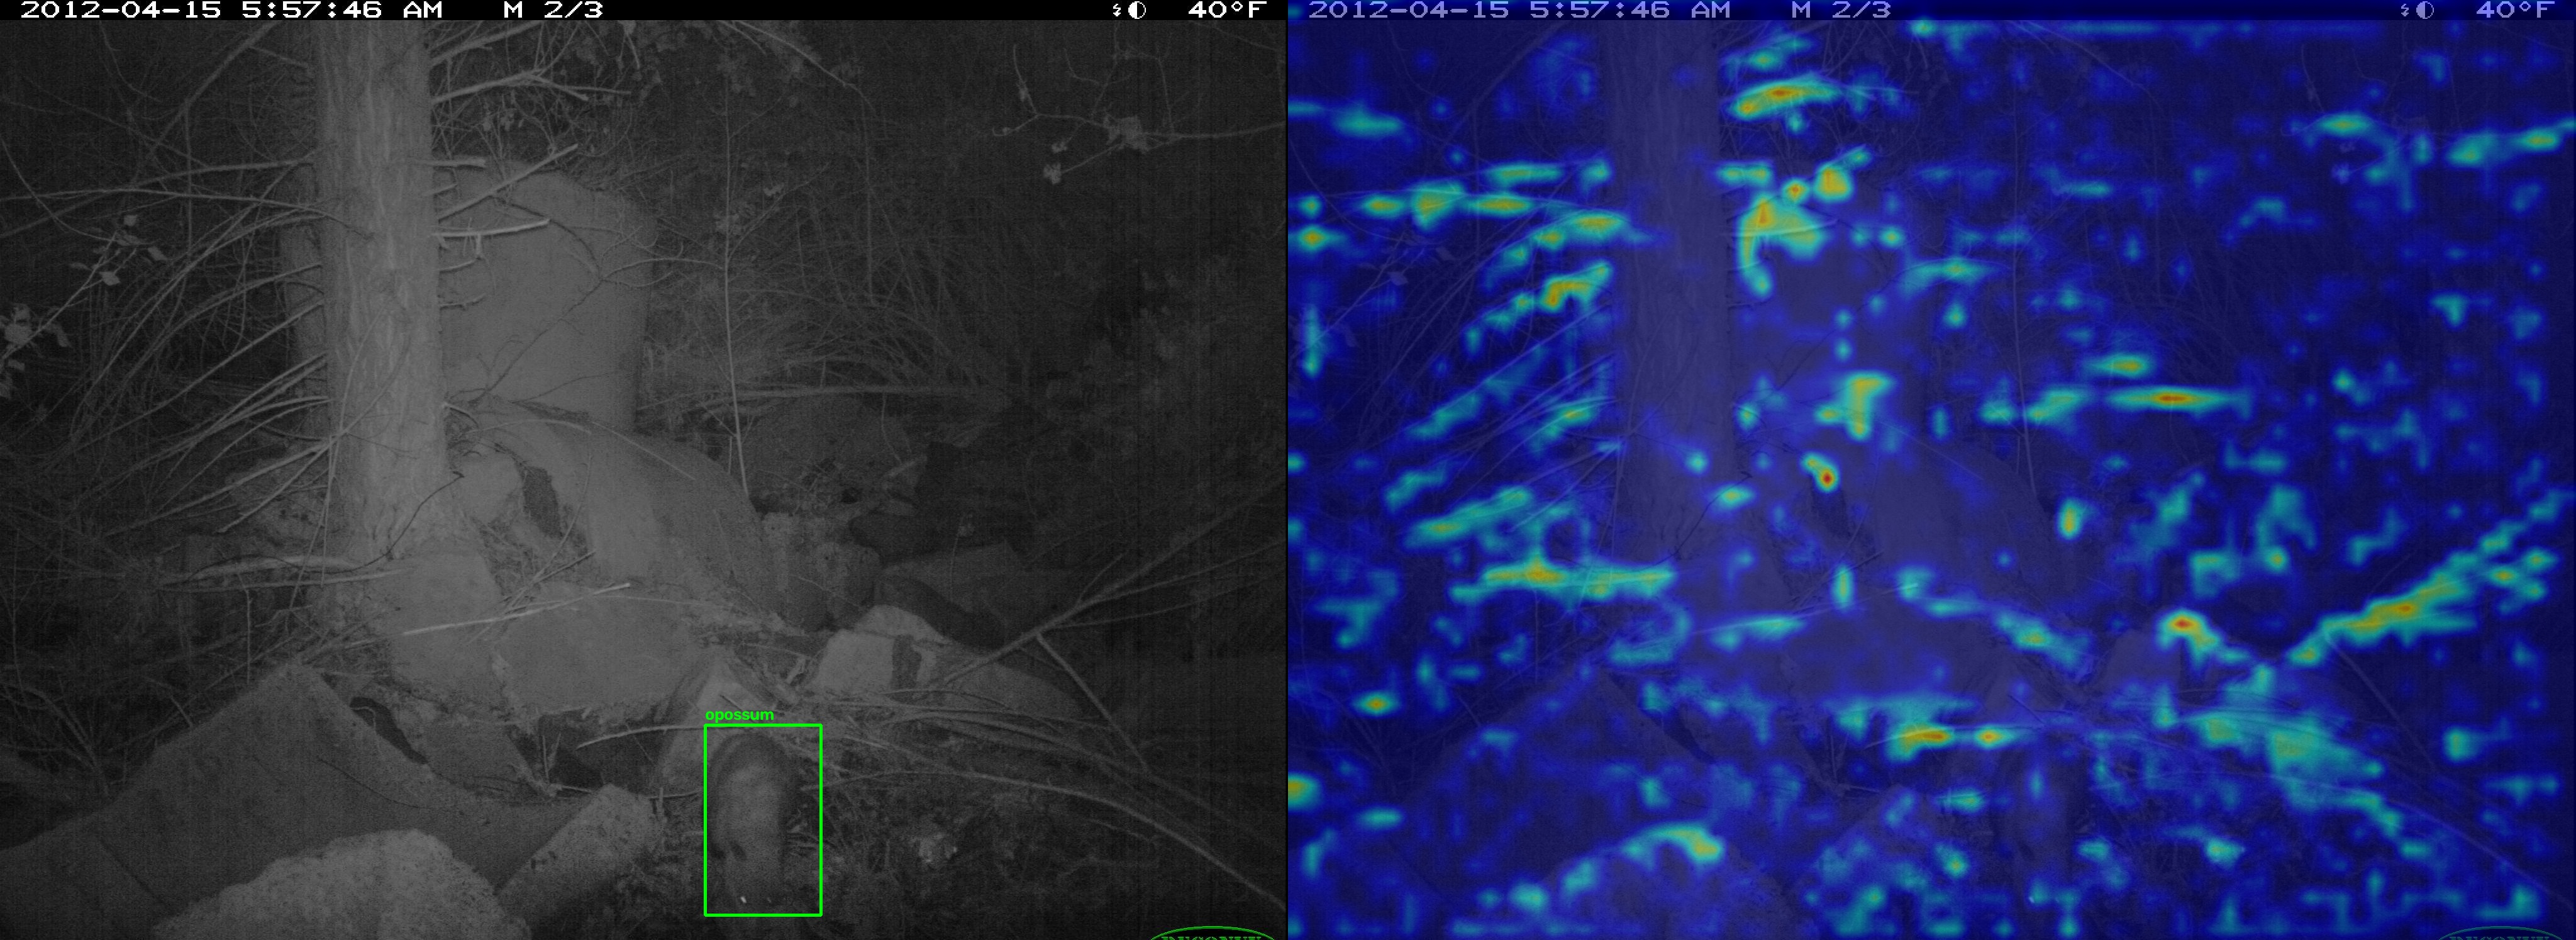
\includegraphics[width=0.5\textwidth]{figuras/trans_test_falso_positivo.jpg}
  \caption{Grad-CAM en una ubicación nunca vista. A la izquierda, la imagen con
    la caja anotada (un \texttt{opossum} al pie de las rocas, abajo al centro);
    a la derecha, el mapa de activación de la clase correcta. La evidencia se
    reparte por la vegetación, las ramas y las rocas de todo el cuadro y apenas
    toca al animal; el modelo no acertó ninguna detección. Es el caso que la
    razón de masa cuantifica: el mapa no está vacío, lo que activa no es el
    animal.}
  \label{fig:gradcam}
\end{figure}

El indicador es la \emph{razón de masa}: qué fracción de la activación cae
dentro de las cajas anotadas, dividida por el área que esas cajas ocupan. Vale
1.0 cuando el mapa es uniforme, es decir cuando el modelo no localiza nada.

Sobre 120 imágenes por partición, la mediana es 1.12 en \texttt{cis\_test} y
1.00 en \texttt{trans\_test}: en la mitad de las imágenes de
ubicaciones nuevas la evidencia del modelo no está más concentrada sobre el
animal que si estuviera repartida al azar. En 52 de 120 imágenes conocidas y 62
de 120 nuevas la razón no supera 1.0.

El desglose por tamaño es más específico y más incómodo. Para animales que
ocupan menos del 1\% del cuadro, la razón es 1.89 en ubicaciones conocidas y
0.89 en ubicaciones nuevas, por debajo de 1.0: la
activación está \emph{menos} concentrada sobre el animal que un mapa uniforme.
Para animales grandes apenas baja, de 1.43 a 1.27. La degradación de
localización se concentra exactamente donde el modelo ya era más débil, y es
coherente con lo que la Sección~\ref{sec:generalizacion} mide con el mAP: en una
cámara nueva, lo que sostenía la detección de un animal chico no estaba en el
animal. La Figura~\ref{fig:gradcam} muestra un caso concreto.

\subsection{Robustez ante tamaño y oclusión}
\label{sec:robustez}

\begin{table}[t]
  \centering
  \footnotesize
  \begin{tabular}{lllrr}
    \toprule
    Barrido & Partición & Nivel & Cajas / imág. & mAP@0.5 \\
    \midrule
    tamaño & \texttt{cis\_test} & diminuto$^{\dagger}$ (0.000--0.00) & 18 & 0.1602 \\
    tamaño & \texttt{cis\_test} & chico (0.002--0.01) & 891 & 0.5131 \\
    tamaño & \texttt{cis\_test} & mediano (0.010--0.05) & 8\,727 & 0.8033 \\
    tamaño & \texttt{cis\_test} & grande (0.050--1.01) & 3\,120 & 0.7341 \\
    tamaño & \texttt{trans\_test} & diminuto$^{\dagger}$ (0.000--0.00) & 16 & 0.0913 \\
    tamaño & \texttt{trans\_test} & chico (0.002--0.01) & 1\,719 & 0.2310 \\
    tamaño & \texttt{trans\_test} & mediano (0.010--0.05) & 11\,878 & 0.4555 \\
    tamaño & \texttt{trans\_test} & grande (0.050--1.01) & 4\,512 & 0.2852 \\
    oclusión & \texttt{cis\textbackslash\{\}\_test} & sin tapar & 1\,500 & 0.7652 \\
    oclusión & \texttt{cis\textbackslash\{\}\_test} & centro, 25\% & 1\,500 & 0.2375 \\
    oclusión & \texttt{cis\textbackslash\{\}\_test} & centro, 50\% & 1\,500 & 0.0584 \\
    oclusión & \texttt{cis\textbackslash\{\}\_test} & centro, 75\% & 1\,500 & 0.0044 \\
    oclusión & \texttt{cis\textbackslash\{\}\_test} & inferior, 25\% & 1\,500 & 0.3699 \\
    oclusión & \texttt{cis\textbackslash\{\}\_test} & inferior, 50\% & 1\,500 & 0.0647 \\
    oclusión & \texttt{cis\textbackslash\{\}\_test} & inferior, 75\% & 1\,500 & 0.0234 \\
    \bottomrule
  \end{tabular}
  \caption{Robustez ante tamaño del objeto y ante oclusión sintética. En el barrido de tamaño, una imagen entra en un tramo solo si \emph{todas} sus cajas caen en el rango —filtrando caja por caja, las descartadas seguirían en la imagen y cada detección correcta de un animal fuera del rango contaría como falso positivo; $^{\dagger}$ menos de 50 cajas. En el de oclusión, el parche tapa la fracción indicada del \emph{área} de cada caja anotada sobre una submuestra fija por semilla: \texttt{centro} deja la silueta y quita la textura, \texttt{inferior} tapa desde el borde de abajo, como la vegetación real, y rompe también la silueta.}
  \label{tab:robustez}
\end{table}


Las imágenes originales son $2048\times1494$ y entran a la red a 640 px, una
reducción de 3.2 veces. Un animal lejano, que ya ocupaba pocos píxeles, queda en
unos pocos. El barrido por tamaño cuantifica ese costo, el caso dominante del
dominio y no una situación marginal.

La oclusión es sintética porque el conjunto no trae esa anotación; la
alternativa era no responder el entregable. El parche tapa la fracción indicada
del \emph{área} de cada caja anotada, y los dos modos no miden lo mismo
(\texttt{centro} deja la silueta y quita la textura; \texttt{inferior} la tapa
desde abajo, como la vegetación real). La interpretación es limpia porque, como
se verificó en la Sección~\ref{sec:metodo_aumento}, el modelo nunca vio oclusión
durante el entrenamiento.

\subsection{Reporte de actividad ecológica}

El entregable \#5 pide demostrar el módulo sobre una cámara no vista en el
entrenamiento, el caso de despliegue real. La demostración principal es por eso
sobre \texttt{trans\_test} (9 cámaras nunca vistas, 2\,090 noches-cámara), con
\texttt{cis\_test} al lado como caso favorable. Las 18\,846 detecciones por
encima de 0.25 se agrupan en 6\,637 eventos independientes (ventana de 30
minutos) contra 4\,819 de las cajas anotadas; en \texttt{cis\_test} son 13\,559
detecciones y 3\,706 eventos. Contar detecciones en vez de eventos habría
inflado la actividad, porque las cámaras disparan ráfagas.

\begin{table}[t]
  \centering
  \footnotesize
  \begin{tabular}{lrrr|rrr}
    \toprule
    Especie & Eventos & Error & Noct. & Eventos & Error & Noct. \\
    \midrule
    \texttt{opossum} & 1\,302 & +14\% & 73\% & 750 & +2\% & 80\% \\
    \texttt{raccoon} & 1\,016 & +15\% & 70\% & 410 & +74\% & 77\% \\
    \texttt{cat} & 786 & +234\% & 46\% & 360 & +21\% & 35\% \\
    \texttt{coyote} & 724 & +30\% & 58\% & 564 & +17\% & 51\% \\
    \texttt{car} & 679 & +12\% & 4\% & 319 & +2\% & 8\% \\
    \texttt{bobcat} & 655 & +13\% & 52\% & 342 & +32\% & 49\% \\
    \texttt{rabbit} & 403 & +108\% & 28\% & 310 & +24\% & 24\% \\
    \texttt{dog} & 309 & +74\% & 7\% & 192 & +42\% & 11\% \\
    \texttt{squirrel} & 252 & +6\% & 2\% & 154 & +18\% & 0\% \\
    \texttt{bird} & 244 & +281\% & 20\% & 139 & +45\% & 12\% \\
    \texttt{skunk} & 226 & +81\% & 71\% & 87 & +12\% & 66\% \\
    \texttt{rodent} & 25 & +150\% & 60\% & 41 & +5\% & 88\% \\
    \texttt{fox} & 9 & +800\% & 89\% & 4 & +100\% & 75\% \\
    \texttt{deer} & 5 & --- & 0\% & 34 & +26\% & 50\% \\
    \texttt{badger} & 2 & -75\% & 100\% & --- & --- & --- \\
    \bottomrule
  \end{tabular}
  \caption{Reporte de actividad por especie. A la izquierda la demostración principal, cámaras nunca vistas (\texttt{trans\_test}: 9 cámaras, 2\,090 noches-cámara); a la derecha el caso favorable, cámaras vistas en el entrenamiento (\texttt{cis\_test}: 10 cámaras, 1\,131 noches-cámara). Un evento independiente agrupa detecciones de la misma especie y cámara separadas por menos de 30 minutos. `Error' es la diferencia relativa de los eventos del modelo contra el mismo reporte calculado desde las cajas anotadas a mano: es la validación del módulo, no un adorno. `Noct.' es el índice de nocturnidad, un control contra la historia natural conocida de cada especie.}
  \label{tab:actividad}
\end{table}


El índice de nocturnidad reproduce la historia natural conocida de las especies
aun en cámaras nuevas, sin recibir esa información: 2\% para \texttt{squirrel},
20\% para \texttt{bird} y 4\% para \texttt{car} (diurnos); 73\% para
\texttt{opossum}, 70\% para \texttt{raccoon} y 71\% para \texttt{skunk}
(nocturnos); 58\% para \texttt{coyote} y 52\% para \texttt{bobcat}
(crepusculares). Es un control que cuesta una columna y detecta errores que el
mAP no ve.

El error contra las anotaciones es lo que decide para qué sirve el módulo. En
\texttt{cis\_test} es siempre positivo y chico, de $+2\%$ a $+100\%$, con las
especies de más datos cerca del valor real (\texttt{opossum} $+2\%$, \texttt{car}
$+2\%$) y las intermedias disparadas (\texttt{raccoon} $+74\%$). En
\texttt{trans\_test} crece (\texttt{cat} $+234\%$, \texttt{bird} $+281\%$) y, a
diferencia de las cámaras conocidas, va en las dos direcciones: \texttt{deer},
sin ninguna caja anotada en esa partición, recibe cinco eventos inventados,
mientras \texttt{badger} se subestima ($-75\%$: ocho eventos anotados, dos
detectados), la especie rara perdida justo donde más importaría registrarla. Esa
tabla de error es el número que un reporte automático debe entregar junto con sus
conclusiones.


\section{Discusión crítica}
\subsection{Qué significa la brecha de 0.35}

El resultado central no es que el modelo generalice mal, que ya lo documentaron
Beery et al.~\cite{beery2018recognition}, sino que ahora se puede decir cuánto
de esa pérdida es realmente por el cambio de ubicación: el control de
distribución descarta la explicación alternativa, porque solo $0.033$ de los
$0.3485$ se explican por el cambio de prevalencia.

El contraste con \texttt{car} es el argumento más fuerte. Si la caída viniera de
un cambio general de dominio (otra cámara, otra iluminación, otro encuadre), el
auto debería caer también. No cae. La diferencia no es el dominio: el auto es
rígido, grande y de alto contraste, mientras que un \texttt{squirrel} a veinte
metros es una mancha que se distingue porque \emph{esa} mancha, en \emph{ese}
tronco, históricamente fue una ardilla.

Grad-CAM lo confirma de forma independiente, y conviene decir hasta dónde. Una
razón de masa mediana de $1.00$ en ubicaciones nuevas no prueba que el modelo
mire el fondo: prueba que su evidencia no está más concentrada sobre el animal
que si estuviera repartida al azar. Es más débil que ``mira el fondo'', pero es
lo que el dato sostiene; para animales chicos ($0.89$) sí cruza el umbral de la
anti-localización.

\subsection{Lo que la métrica agregada no puede expresar}

El caso de \texttt{deer} en \texttt{trans\_test} es instructivo más allá de este
trabajo: cero cajas anotadas y 646 detecciones emitidas. La AP no está definida y
se reporta como tal, pero ningún valor de AP (ni cero, ni indefinido) comunica
que el modelo inventa ciervos. Con \texttt{bird} pasa el caso inverso: 17\,086
detecciones para 180 cajas y AP $= 0.0132$, que un lector entiende como ``no
detecta pájaros'' cuando el problema es el exceso de detecciones. De ahí que la
tabla por especie incluya las detecciones junto al soporte: convierte un AP bajo
en un diagnóstico, porque con pocas detecciones es falta de recall y con muchas,
de precisión, y las dos se arreglan distinto.

\subsection{Decisiones que podrían haber salido de otra forma}

\emph{La resolución.} 640 px se tomó porque es la de los pesos preentrenados y
permite un lote de 16. El barrido por tamaño muestra su costo; el experimento que
lo cerraría, reentrenar a 960 px, no se hizo, así que se afirma el diagnóstico y
no la mitigación.

\emph{El tramo grande rinde peor que el mediano}, en las dos particiones
($0.7341$ contra $0.8033$, y $0.2852$ contra $0.4555$), y no era lo esperado. La
hipótesis plausible es que un animal que ocupa más del 5\% del cuadro está muy
cerca del lente: entra parcialmente fuera de cuadro, con desenfoque de movimiento
y, de noche, sobreexpuesto por el infrarrojo. Cuál domina no se midió, así que
queda como observación.

\emph{Una predicción equivocada sobre la oclusión.} Se diseñó el modo
\texttt{inferior} esperando que fuera el caso más duro, porque rompe la silueta
además de tapar la textura. Medido, al 25\% es claramente más benigno que tapar
el centro ($0.3699$ contra $0.2375$): el modelo se apoya más en la textura
interior que en el contorno, y al 50\% la diferencia se desvanece. Se registra
porque la hipótesis estaba escrita antes de medir.

\emph{Los negativos explícitos.} Las imágenes vacías podrían sumarse como
fondo; no se hizo porque habría cambiado a la vez el tamaño del conjunto y la
proporción fondo/objeto. Dado el volumen de falsos positivos en terreno nuevo,
es la ablación pendiente más prometedora.

\subsection{Límites de lo que se midió}

\emph{Una sola corrida de entrenamiento.} Los intervalos de confianza
capturan la variabilidad del \emph{muestreo de imágenes}, no la de la
\emph{inicialización}: no se entrenaron varias semillas. La brecha de $0.35$ es
mucho mayor que cualquier variación por semilla plausible, pero las diferencias
chicas de este informe, como el tramo grande contra el mediano, no se pueden
atribuir con esa evidencia.

\emph{La oclusión es sintética.} Un rectángulo gris uniforme es más fácil de
ignorar, o de confundir, que una rama real con textura. La dirección del
resultado es contundente; su magnitud exacta no se traslada a oclusión natural.

\emph{La ocupación del módulo ecológico es naive} y debe leerse como cota
inferior. El error del reporte se midió sobre las dos particiones: en
\texttt{cis\_test}, el caso favorable, va de $+2\%$ a $+100\%$ y siempre
sobreestima; en \texttt{trans\_test} es mayor, hasta $+281\%$ en \texttt{bird}, y
aparece en las dos direcciones, porque el modelo inventa eventos de las especies
comunes y a la vez pierde los de \texttt{badger} ($-75\%$), la rara.


\section{Uso responsable de IA en conservación}
\label{sec:responsable}

Los resultados de este trabajo son, en sí mismos, el argumento de por qué un
detector de fauna no debe desplegarse como oráculo. Tres de ellos lo dicen con
números propios.

\emph{El desempeño se derrumba fuera de las cámaras conocidas.} La brecha entre
ubicaciones vistas y nuevas (Sección~\ref{sec:generalizacion}) significa que
validar un modelo en las cámaras donde se entrenó sobreestima lo que hará en una
cámara nueva. Un proyecto que instala un sensor en un sitio no muestreado y
confía en la cifra de validación está usando un número que no corresponde a su
situación. La consecuencia operativa es concreta: las métricas que se publican
junto a un modelo de este dominio deben declarar en qué ubicaciones se midieron.

\emph{El error no es uniforme entre especies, y es peor donde más importa.} Las
especies con menos datos de entrenamiento son las que el modelo detecta peor, y
suelen ser también las de mayor interés para conservación, las raras. Los dos
errores no cuestan lo mismo en este dominio: un falso negativo, no registrar una
especie rara que sí estaba, puede hacer concluir que un sitio está vacío y
justificar no protegerlo, mientras que un falso positivo cuesta sobre todo tiempo
de verificación humana; el daño se concentra justo donde el modelo es más débil.
Un reporte automático subestima sistemáticamente a las especies cuya presencia o
ausencia puede motivar una decisión de manejo. Reportar un único mAP agregado
oculta ese sesgo; por eso el desglose por especie con su soporte al lado no es un
detalle de presentación sino una condición para que el número sea utilizable.

\emph{El modelo no mira donde uno supone.} La razón de masa de Grad-CAM
(Sección~\ref{sec:gradcam}) muestra que buena parte de la evidencia que el modelo
usa no cae sobre el animal. Un sistema que acierta apoyándose en el fondo acierta
hasta que el fondo cambia, y no hay nada en su salida que avise cuándo eso
ocurrió. La confianza que el detector reporta no es una medida de que esté
mirando lo correcto.

De ahí, cuatro compromisos para un despliegue responsable, respaldados por las
mediciones de este trabajo.

\emph{Asistir, no decidir.} El uso defendible es el que MegaDetector adoptó
explícitamente~\cite{beery2019efficient}: filtrar el volumen de imágenes vacías,
que es el trabajo tedioso, y dejar la identificación de especie a revisión
humana, especialmente en las especies raras, donde el modelo es menos fiable y el
costo de un error es mayor.

\emph{Declarar la incertidumbre junto al número.} Un conteo de eventos sin su
error invita a conclusiones que no aguanta; por eso el módulo de monitoreo
reporta su error especie por especie contra las anotaciones humanas, en vez de
dejar que el lector lo suponga.

\emph{Cuidar el dato de ubicación.} Las coordenadas de las cámaras trampa son
información sensible: un registro de dónde y cuándo aparece una especie amenazada
es lo que necesita quien quiera cazarla. Un pipeline que indexa y publica
detecciones amplifica ese riesgo a escala, así que lo que se comparte debe ir
agregado o con la ubicación degradada deliberadamente.

\emph{No confundir ausencia de detección con ausencia de animal.} La ocupación
que el módulo del entregable \#5 reporta es \emph{naive}: una especie presente
pero no fotografiada cuenta como ausente. Corregirlo exige modelar la
probabilidad de detección~\cite{mackenzie2002estimating}, y mientras no se haga,
la cifra es una cota inferior, no una estimación. Decirlo es parte del reporte,
no una advertencia al pie: una ocupación subestimada puede justificar la decisión
de no proteger un sitio.


\section{Conclusiones}
Un detector YOLO11 ajustado sobre Caltech Camera Traps alcanza mAP@0.5
$= 0.7463$ donde se entrenó y $0.3978$ en ubicaciones nuevas. La brecha de
$0.3485$ sobrevive al control del cambio de prevalencia (que explica solo
$0.033$) y no afecta a todas las clases por igual: \texttt{car}, el único objeto
rígido, conserva su desempeño mientras los animales pierden entre un tercio y el
98\% de su AP. Lo que falla no es el cambio de dominio sino la evidencia
específica con que se reconoce al animal.

Grad-CAM, con la capa elegida por medición y no por convención, da una medida
independiente: en la mitad de las imágenes nuevas la activación no supera a un
mapa uniforme, y para los animales bajo el 1\% del cuadro queda por debajo. La
robustez ante oclusión es nula (tapar un cuarto del área cuesta dos tercios del
mAP), sobre un modelo que —verificado— nunca vio oclusión, pese a lo que sugiere
el registro de la corrida.

El módulo de monitoreo, demostrado sobre cámaras nunca vistas, produce un reporte
cuyo índice de nocturnidad reproduce la historia natural de las especies sin
recibir esa información, y que a la vez se desvía en el conteo de casi todas
(hasta $+281\%$ en \texttt{bird}, $+800\%$ en \texttt{fox} con un solo evento
anotado): captura la señal ecológica gruesa pero no la magnitud, y por eso
publica su error contra las anotaciones humanas.

Quedan tres líneas de trabajo: reentrenar a 960 px, sumar las imágenes vacías
como negativos y entrenar varias semillas para atribuir las diferencias pequeñas.


\section*{Reproducibilidad}
Todo se reproduce con un único comando, \texttt{python
pregunta3/paso7\_informe/ejecutar\_todo.py} (en el README), que va de la descarga
a este documento y se retoma sin repetir lo hecho. Las 113 pruebas propias
(\texttt{tests/test\_p3\_*.py}) fijan la definición de AP y la agrupación en
eventos.

{\small
\bibliographystyle{plain}
\bibliography{referencias}
}

\end{document}
